%************************************************
\chapter{Deep Generative Models}\label{ch:dgms}
%************************************************

Let us start with the definition of our dataset $\mathcal{D}$, consisting of $N \geq 1$ data points, where the instances are assumed to be independently and 
identically distributed. Assume $\mathbf{x}$ represents the set of observed variables (images in our case), which is a random sample from an unknown underlying 
process, whose true distribution $p^*(\mathbf{x})$ is unknown. The idea is to approximate the real process with a model $p_{\theta}(\mathbf{x})$ with parameters 
$\theta$. Learning has the aim of finding a value of parameters $\theta$ such that the probability distribution of the model, $p_{\theta}(\mathbf{x})$, approximates 
the true distribution for any observed set of variables, i.e. $p_{\theta}(\mathbf{x}) \approx p^*(\mathbf{x})$. \\
\\
Deep Generative Models (DGMs) are neural networks that are a flexible way to parameterise distributions that learn $p_{\theta}(\mathbf{x})$, which is commonly 
referred to as a generative model. Once the model is available, we can generate new samples using sampling methods and compute the likelihood of any given data 
point $\mathbf{x}'$ by evaluating $p_{\theta}(\mathbf{x}')$.   

\section{Training of DGM} 

The general idea is to learn the parameters $\theta$ by minimizing the discrepancy between real and predicted data distribution: 
$$\theta^{*} = \arg\min_{\theta} \mathcal{D}(p_{data}, p_{\theta}).$$ Because $p_{data}$ is unknown, we have to choose a discrepancy function that allows efficient 
estimation from samples from $p_{data}$. 

\begin{figure}
    \centering
    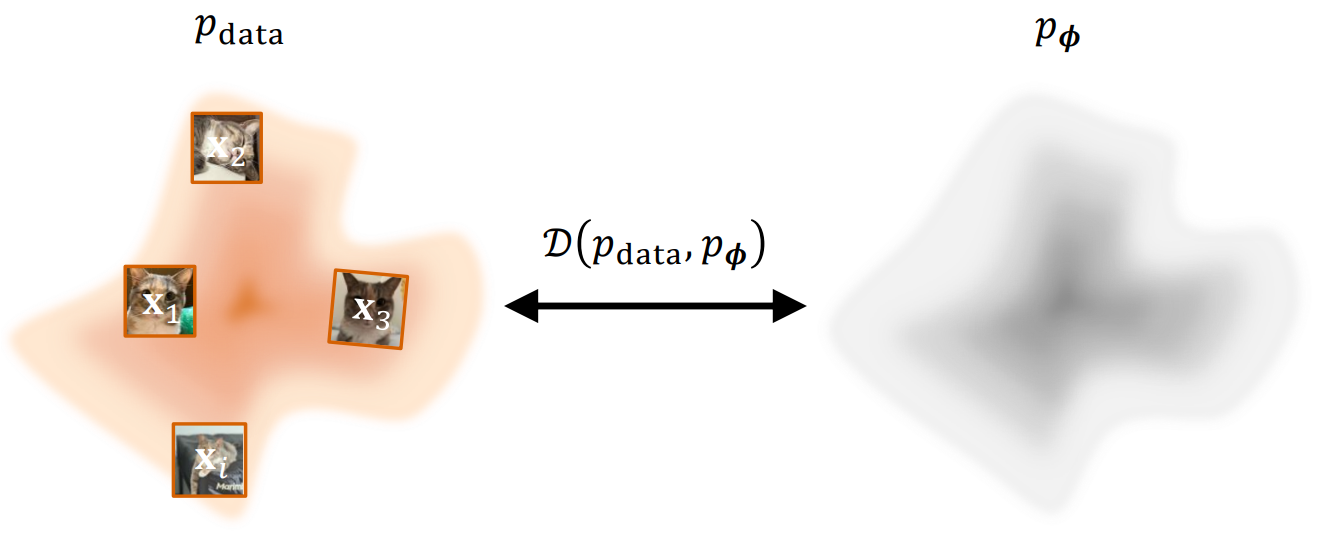
\includegraphics[width=0.8\linewidth]{gfx/dgm/dgm1.png}
    \caption{Visualization of the training of DGMs where we minimize a discrepancy measure between the real and unknown data distribution and the approximated one, using a set of i.i.d. samples.\cite{lai2025principlesdiffusionmodels}}
    \label{fig:dgm1}
\end{figure}

The most common choice is the Kullback-Leibler divergence, defined as 
\begin{equation}
\begin{split}
    \mathcal{D}_{KL}(p_{data}||p_{\theta}) = \int p_{data}(\mathbf{x})\log \frac{p_{data}(\mathbf{x})}{p_{\theta}(\mathbf{x})}d\mathbf{x} = \\ 
    \mathbb{E}_{\mathbf{x}\sim p_{data}}\left[\log p_{data}(\mathbf{x}) - \log p_{\theta}(\mathbf{x})\right],
\end{split}
\end{equation}
where, taking into account only the part that depends 
on the parameter $\theta$, minimizing the KL divergence is equivalent to performing MLE: $$\min_{\theta}\mathcal{D}_{KL}(p_{data}||p_{\theta}) \Longleftrightarrow 
\max_{\theta}\mathbb{E}_{\mathbf{x}\sim p_{data}}\left[\log p_{\theta}(\mathbf{x})\right].$$ In practice, we do not have access to the data distribution, only to 
some i.i.d. samples $\{\mathbf{x}^{(i)}\}_{i=1}^N\sim p_{data}$, which are used to obtain the empirical estimate of the MSE $$\mathcal{L}_{MLE}(\theta) = 
-\frac{1}{N}\sum_{i=1}^N\log p_{\theta}(\mathbf{x}^{(i)}).$$   
There are some challenges in the use of neural networks to parameterize the probability distribution $p_{data}$. We can define a model that produces a real scalar 
$E_{\theta}(\mathbf{x})\in\mathbb{R}$ for input $\mathbf{x}$. To interpret the output as a valid probability density, it has to satisfy the following conditions: 
\begin{itemize}
    \item \textbf{Non-Negativity}: $p_{\theta}(\mathbf{x})\geq 0$ for all $\mathbf{x}$ in the domain. The standard positive function is used to guarantee non-negativity 
    is the exponential function, which produces an unnormalized density $\tilde p_{\theta}(\mathbf{x}) = \exp(E_{\theta}(\mathbf{x}))$.
    \item \textbf{Normalization}: The integral over the entire domain must equal one. To create a valid probability density, we must divide it by its integral over 
    the entire space $$p_{\theta}(\mathbf{x})=\frac{\tilde p_{\theta}(\mathbf{x})}{Z(\theta)},$$ where the denominator is the partition function defined as 
    $$Z(\theta)=\int \tilde p_{\theta}(\mathbf{x'})d\mathbf{x'}.$$ 
\end{itemize}
The partition function introduces a computational challenge in the learning of probabilistic models, especially for high-dimensional problems. This intractability is 
a central problem that motivates the development of many different families of deep generative models, which will be explained in the following chapters. 


%*****************************************
%*****************************************
%*****************************************
%*****************************************
%*****************************************